% Options for packages loaded elsewhere
\PassOptionsToPackage{unicode}{hyperref}
\PassOptionsToPackage{hyphens}{url}
%
\documentclass[
  ignorenonframetext,
]{beamer}
\usepackage{pgfpages}
\setbeamertemplate{caption}[numbered]
\setbeamertemplate{caption label separator}{: }
\setbeamercolor{caption name}{fg=normal text.fg}
\beamertemplatenavigationsymbolsempty
% Prevent slide breaks in the middle of a paragraph
\widowpenalties 1 10000
\raggedbottom
\setbeamertemplate{part page}{
  \centering
  \begin{beamercolorbox}[sep=16pt,center]{part title}
    \usebeamerfont{part title}\insertpart\par
  \end{beamercolorbox}
}
\setbeamertemplate{section page}{
  \centering
  \begin{beamercolorbox}[sep=12pt,center]{part title}
    \usebeamerfont{section title}\insertsection\par
  \end{beamercolorbox}
}
\setbeamertemplate{subsection page}{
  \centering
  \begin{beamercolorbox}[sep=8pt,center]{part title}
    \usebeamerfont{subsection title}\insertsubsection\par
  \end{beamercolorbox}
}
\AtBeginPart{
  \frame{\partpage}
}
\AtBeginSection{
  \ifbibliography
  \else
    \frame{\sectionpage}
  \fi
}
\AtBeginSubsection{
  \frame{\subsectionpage}
}

\usepackage{amsmath,amssymb}
\usepackage{iftex}
\ifPDFTeX
  \usepackage[T1]{fontenc}
  \usepackage[utf8]{inputenc}
  \usepackage{textcomp} % provide euro and other symbols
\else % if luatex or xetex
  \usepackage{unicode-math}
  \defaultfontfeatures{Scale=MatchLowercase}
  \defaultfontfeatures[\rmfamily]{Ligatures=TeX,Scale=1}
\fi
\usepackage{lmodern}
\usetheme[]{metropolis}
\ifPDFTeX\else  
    % xetex/luatex font selection
\fi
% Use upquote if available, for straight quotes in verbatim environments
\IfFileExists{upquote.sty}{\usepackage{upquote}}{}
\IfFileExists{microtype.sty}{% use microtype if available
  \usepackage[]{microtype}
  \UseMicrotypeSet[protrusion]{basicmath} % disable protrusion for tt fonts
}{}
\makeatletter
\@ifundefined{KOMAClassName}{% if non-KOMA class
  \IfFileExists{parskip.sty}{%
    \usepackage{parskip}
  }{% else
    \setlength{\parindent}{0pt}
    \setlength{\parskip}{6pt plus 2pt minus 1pt}}
}{% if KOMA class
  \KOMAoptions{parskip=half}}
\makeatother
\usepackage{xcolor}
\newif\ifbibliography
\setlength{\emergencystretch}{3em} % prevent overfull lines
\setcounter{secnumdepth}{-\maxdimen} % remove section numbering

\usepackage{color}
\usepackage{fancyvrb}
\newcommand{\VerbBar}{|}
\newcommand{\VERB}{\Verb[commandchars=\\\{\}]}
\DefineVerbatimEnvironment{Highlighting}{Verbatim}{commandchars=\\\{\}}
% Add ',fontsize=\small' for more characters per line
\usepackage{framed}
\definecolor{shadecolor}{RGB}{241,243,245}
\newenvironment{Shaded}{\begin{snugshade}}{\end{snugshade}}
\newcommand{\AlertTok}[1]{\textcolor[rgb]{0.68,0.00,0.00}{#1}}
\newcommand{\AnnotationTok}[1]{\textcolor[rgb]{0.37,0.37,0.37}{#1}}
\newcommand{\AttributeTok}[1]{\textcolor[rgb]{0.40,0.45,0.13}{#1}}
\newcommand{\BaseNTok}[1]{\textcolor[rgb]{0.68,0.00,0.00}{#1}}
\newcommand{\BuiltInTok}[1]{\textcolor[rgb]{0.00,0.23,0.31}{#1}}
\newcommand{\CharTok}[1]{\textcolor[rgb]{0.13,0.47,0.30}{#1}}
\newcommand{\CommentTok}[1]{\textcolor[rgb]{0.37,0.37,0.37}{#1}}
\newcommand{\CommentVarTok}[1]{\textcolor[rgb]{0.37,0.37,0.37}{\textit{#1}}}
\newcommand{\ConstantTok}[1]{\textcolor[rgb]{0.56,0.35,0.01}{#1}}
\newcommand{\ControlFlowTok}[1]{\textcolor[rgb]{0.00,0.23,0.31}{#1}}
\newcommand{\DataTypeTok}[1]{\textcolor[rgb]{0.68,0.00,0.00}{#1}}
\newcommand{\DecValTok}[1]{\textcolor[rgb]{0.68,0.00,0.00}{#1}}
\newcommand{\DocumentationTok}[1]{\textcolor[rgb]{0.37,0.37,0.37}{\textit{#1}}}
\newcommand{\ErrorTok}[1]{\textcolor[rgb]{0.68,0.00,0.00}{#1}}
\newcommand{\ExtensionTok}[1]{\textcolor[rgb]{0.00,0.23,0.31}{#1}}
\newcommand{\FloatTok}[1]{\textcolor[rgb]{0.68,0.00,0.00}{#1}}
\newcommand{\FunctionTok}[1]{\textcolor[rgb]{0.28,0.35,0.67}{#1}}
\newcommand{\ImportTok}[1]{\textcolor[rgb]{0.00,0.46,0.62}{#1}}
\newcommand{\InformationTok}[1]{\textcolor[rgb]{0.37,0.37,0.37}{#1}}
\newcommand{\KeywordTok}[1]{\textcolor[rgb]{0.00,0.23,0.31}{#1}}
\newcommand{\NormalTok}[1]{\textcolor[rgb]{0.00,0.23,0.31}{#1}}
\newcommand{\OperatorTok}[1]{\textcolor[rgb]{0.37,0.37,0.37}{#1}}
\newcommand{\OtherTok}[1]{\textcolor[rgb]{0.00,0.23,0.31}{#1}}
\newcommand{\PreprocessorTok}[1]{\textcolor[rgb]{0.68,0.00,0.00}{#1}}
\newcommand{\RegionMarkerTok}[1]{\textcolor[rgb]{0.00,0.23,0.31}{#1}}
\newcommand{\SpecialCharTok}[1]{\textcolor[rgb]{0.37,0.37,0.37}{#1}}
\newcommand{\SpecialStringTok}[1]{\textcolor[rgb]{0.13,0.47,0.30}{#1}}
\newcommand{\StringTok}[1]{\textcolor[rgb]{0.13,0.47,0.30}{#1}}
\newcommand{\VariableTok}[1]{\textcolor[rgb]{0.07,0.07,0.07}{#1}}
\newcommand{\VerbatimStringTok}[1]{\textcolor[rgb]{0.13,0.47,0.30}{#1}}
\newcommand{\WarningTok}[1]{\textcolor[rgb]{0.37,0.37,0.37}{\textit{#1}}}

\providecommand{\tightlist}{%
  \setlength{\itemsep}{0pt}\setlength{\parskip}{0pt}}\usepackage{longtable,booktabs,array}
\usepackage{calc} % for calculating minipage widths
\usepackage{caption}
% Make caption package work with longtable
\makeatletter
\def\fnum@table{\tablename~\thetable}
\makeatother
\usepackage{graphicx}
\makeatletter
\def\maxwidth{\ifdim\Gin@nat@width>\linewidth\linewidth\else\Gin@nat@width\fi}
\def\maxheight{\ifdim\Gin@nat@height>\textheight\textheight\else\Gin@nat@height\fi}
\makeatother
% Scale images if necessary, so that they will not overflow the page
% margins by default, and it is still possible to overwrite the defaults
% using explicit options in \includegraphics[width, height, ...]{}
\setkeys{Gin}{width=\maxwidth,height=\maxheight,keepaspectratio}
% Set default figure placement to htbp
\makeatletter
\def\fps@figure{htbp}
\makeatother
\newlength{\cslhangindent}
\setlength{\cslhangindent}{1.5em}
\newlength{\csllabelwidth}
\setlength{\csllabelwidth}{3em}
\newlength{\cslentryspacingunit} % times entry-spacing
\setlength{\cslentryspacingunit}{\parskip}
\newenvironment{CSLReferences}[2] % #1 hanging-ident, #2 entry spacing
 {% don't indent paragraphs
  \setlength{\parindent}{0pt}
  % turn on hanging indent if param 1 is 1
  \ifodd #1
  \let\oldpar\par
  \def\par{\hangindent=\cslhangindent\oldpar}
  \fi
  % set entry spacing
  \setlength{\parskip}{#2\cslentryspacingunit}
 }%
 {}
\usepackage{calc}
\newcommand{\CSLBlock}[1]{#1\hfill\break}
\newcommand{\CSLLeftMargin}[1]{\parbox[t]{\csllabelwidth}{#1}}
\newcommand{\CSLRightInline}[1]{\parbox[t]{\linewidth - \csllabelwidth}{#1}\break}
\newcommand{\CSLIndent}[1]{\hspace{\cslhangindent}#1}

\usepackage{linguex}
\usepackage{qtree}
\usepackage{stmaryrd}
\usepackage{hyperref}
\newcommand{\sem}[1]{\llbracket{\mathrm{#1}}\rrbracket}
\renewcommand{\eachwordone}{\small}
\renewcommand{\eachwordtwo}{\small}
\newcommand{\cond}[1]{\textsc{#1}}
\makeatletter
\makeatother
\makeatletter
\makeatother
\makeatletter
\@ifpackageloaded{caption}{}{\usepackage{caption}}
\AtBeginDocument{%
\ifdefined\contentsname
  \renewcommand*\contentsname{Table of contents}
\else
  \newcommand\contentsname{Table of contents}
\fi
\ifdefined\listfigurename
  \renewcommand*\listfigurename{List of Figures}
\else
  \newcommand\listfigurename{List of Figures}
\fi
\ifdefined\listtablename
  \renewcommand*\listtablename{List of Tables}
\else
  \newcommand\listtablename{List of Tables}
\fi
\ifdefined\figurename
  \renewcommand*\figurename{Figure}
\else
  \newcommand\figurename{Figure}
\fi
\ifdefined\tablename
  \renewcommand*\tablename{Table}
\else
  \newcommand\tablename{Table}
\fi
}
\@ifpackageloaded{float}{}{\usepackage{float}}
\floatstyle{ruled}
\@ifundefined{c@chapter}{\newfloat{codelisting}{h}{lop}}{\newfloat{codelisting}{h}{lop}[chapter]}
\floatname{codelisting}{Listing}
\newcommand*\listoflistings{\listof{codelisting}{List of Listings}}
\makeatother
\makeatletter
\@ifpackageloaded{caption}{}{\usepackage{caption}}
\@ifpackageloaded{subcaption}{}{\usepackage{subcaption}}
\makeatother
\makeatletter
\@ifpackageloaded{tcolorbox}{}{\usepackage[skins,breakable]{tcolorbox}}
\makeatother
\makeatletter
\@ifundefined{shadecolor}{\definecolor{shadecolor}{rgb}{.97, .97, .97}}
\makeatother
\makeatletter
\makeatother
\makeatletter
\makeatother
\ifLuaTeX
  \usepackage{selnolig}  % disable illegal ligatures
\fi
\IfFileExists{bookmark.sty}{\usepackage{bookmark}}{\usepackage{hyperref}}
\IfFileExists{xurl.sty}{\usepackage{xurl}}{} % add URL line breaks if available
\urlstyle{same} % disable monospaced font for URLs
\hypersetup{
  pdftitle={Grammatical and demographic factors in linguistics},
  pdfauthor={Mojmír Dočekal},
  hidelinks,
  pdfcreator={LaTeX via pandoc}}

\title{Grammatical and demographic factors in linguistics}
\subtitle{experimental evidence from Czech equatives}
\author{Mojmír Dočekal}
\date{11-05-2023}
\institute{Innsbruck}

\begin{document}
\frame{\titlepage}
\ifdefined\Shaded\renewenvironment{Shaded}{\begin{tcolorbox}[breakable, boxrule=0pt, frame hidden, enhanced, sharp corners, interior hidden, borderline west={3pt}{0pt}{shadecolor}]}{\end{tcolorbox}}\fi

\begin{frame}{Intro}
\protect\hypertarget{intro}{}
\begin{itemize}
\tightlist
\item
  talk about expressions depending on the polarity
\item
  evidence: Czech (strict negative concord language)
\item
  data gathered from many experiments: long and extensive collaborative
  work with Jakub Dotlačil, Iveta Šafratová, Tereza Slunská, Martin
  Juřen and many other linguists in Brno and around
\item
  add to experimental research on NPIs: Chemla, Homer, and Rothschild
  (2011),J. Gajewski (2016),Alexandropoulou, Bylinina, and Nouwen (2020)
  a.o.
\item
  more specifically: Djärv, Zehr, and Schwarz (2018),Schwarz, Djärv, and
  Zehr (2020) and their experimental work on cross-linguistic variation
  in NPI licensing (following Chierchia (2019))
\end{itemize}
\end{frame}

\begin{frame}
\begin{block}{Negative polarity items vs.~neg-words}
\protect\hypertarget{negative-polarity-items-vs.-neg-words}{}
\begin{itemize}
\tightlist
\item
  Negative polarity items (English \emph{any}) require negation or such
  operators which share with negation the downward entailing property
\end{itemize}

\ex. \a. John doesn't like cats. \b. \(\rightarrow\) John doesn't like
black cats. \c. John doesn't like \textbf{any} cats.

\ex. \a. If you like cats buy this book. \b. \(\rightarrow\) If you like
black cats buy this book. \c. If you like \textbf{any cats} buy this
book.

~
\end{block}
\end{frame}

\begin{frame}
\begin{block}{Neg-words}
\protect\hypertarget{neg-words}{}
\begin{itemize}
\tightlist
\item
  expressions like Italian \emph{nessuno} requiring negation on verb
\end{itemize}

\ex. A John non piace nessuno.\\
John doesn't like anybody.

\begin{itemize}
\tightlist
\item
  in Slavic languages (like in Romance languages) negative pronouns
  roughly corresponding to \emph{anybody}, \emph{anything},
  \emph{anywhere}, \ldots{}
\end{itemize}
\end{block}
\end{frame}

\begin{frame}
Czech neg-words

\begin{itemize}
\tightlist
\item
  similar to Italian neg-words (\emph{niente}, e.g.: Ladusaw (1992)) but
  as in all Slavic languages (strict negative-concord: Zeijlstra (2004))
  in majority of contexts require verbal negation (in the same clause)
\end{itemize}

\ex. \ag. Petr nedal žádný gól.\\
Petr neg-scored neg-word goal\\
`Petr didn't score any goal.\textquotesingle{} \bg. Nikdo
\{nepřišel/\#přišel\}.\\
neg-word neg-came/came\\
`Nobody came.' \cg. *Petr neřekl, že nikdo přišel.\\
Petr neg-said that neg-word came\\
\hspace*{0.333em}

~
\end{frame}

\begin{frame}
\begin{itemize}
\tightlist
\item
  empirically, the talk is about Czech strong NPIs and neg-words
\item
  \emph{ani jeden} `even one' vs.~\textit{žádný} `no' (neg-word)
\item
  in the majority of contexts: interchangeable -- \Next
\end{itemize}

\exg. Petr nepotkal \{ani jednoho/žádného\} studenta.\\
Petr neg-met strong NPI/neg-word student\\
`Petr didn't meet even one/any student.'

\begin{itemize}
\tightlist
\item
  strong NPIs (theoretical framework: Jon R. Gajewski (2011)) but with
  the unlikelihood presupposition (English \emph{ANY}: Krifka (1995),
  Hindi \emph{ek bhii}: Lahiri (1998), English \emph{even one}: Crnič
  (2014b))
\end{itemize}
\end{frame}

\begin{frame}
\begin{itemize}
\tightlist
\item
  \emph{ani}: the unlikelihood presupposition of English \emph{even} but
  limited to strong NPI contexts
\item
  strongest (unlikely) prejacent: entailing all the alternatives
\end{itemize}

\exg. FC Barcelona nedala \{ani jeden/\#ani deset\} gól/ů.\\
FC Barcelona neg-gave even one/\#even ten goal(s)\\
`FC Barcelona didn't score even one/\#ten goal(s).'

~
\end{frame}

\begin{frame}
\begin{itemize}
\tightlist
\item
  the most influential analysis of neg-words: syntactic approach
  (Zeijlstra (2004) a.o.)
\item
  in strict negative concord languages, all neg-words (and the verbal)
  negation carry {[}uNeg{]} and are checked against {[}iNeg{]} (covert)
  operator with the semantics of \(\neg\)
\item
  part of the talk: experimental support for an alternative, semantic
  theory of neg-words (Ovalle and Guerzoni (2004),Kuhn (2022))
\end{itemize}
\end{frame}

\begin{frame}
\begin{itemize}
\tightlist
\item
  equatives: one of the contexts where strong NPIs and neg-words
  distribution diverge
\item
  Czech equatives don't license strong \& weak NPIs (like German and
  many other non-English NPIs: see Krifka (1992)) but license neg-words
\item
  surprising against English and standard theories of equatives Stechow
  (1984),Beck (2019) a.o.
\item
  one of the environments where the contrast is most robust but still
  there's a variation: some speakers treat \emph{ani} as neg-word
\end{itemize}

\exg. Petr je tak vysoký jako \{\#ani jeden/žádný\} jiný student.\\
Petr is so tall how strong NPI/neg-word other student.\\
\hspace*{0.333em}

\ex. Paris is as quiet as ever.

~
\end{frame}

\begin{frame}
\begin{block}{Bigger picture}
\protect\hypertarget{bigger-picture}{}
\begin{itemize}
\tightlist
\item
  English NPIs vs.~negative quantifiers
\item
  previous studies (typology, functional linguistics -- Tottie (1991)
  a.o.): the newer NPIs replace the older negative quantifiers
\item
  Burnett, Koopman, and Tagliamonte (2018): NPIs replace negative
  quantifiers in some (lower, e.g.) syntactic domains

  \begin{itemize}
  \tightlist
  \item
    historical and social factors are real but weaker than grammatical
  \end{itemize}
\end{itemize}

\ex. \a. I know nothing. \hfill negative quant.\\
\b. I don't know anything. \hfill NPI

\begin{itemize}
\tightlist
\item
  similarly: Burnett, Tremblay, and Blondeau (2015): the variable
  negative concord in Québec French
\item
  is not only explainable by social factors (age, education): against
  older sociolinguistic work
\end{itemize}
\end{block}
\end{frame}

\begin{frame}
\begin{itemize}
\tightlist
\item
  this talk: is also about the variation

  \begin{itemize}
  \tightlist
  \item
    for a diachronic glimpse: Appendix
  \end{itemize}
\item
  similar to Burnett, Tremblay, and Blondeau (2015): the distinction
  between neg-words and strong NPIs is robust and well testable

  \begin{itemize}
  \tightlist
  \item
    nothing like a historical replacement of the older strong NPIs by
    newer neg-words
  \end{itemize}
\item
  but there is a change in process: some speakers use strong NPIs as
  neg-words
\item
  experimental work: search for factors (grammatical and social as well)
\item
  plus explaining the puzzling equative pattern
\end{itemize}
\end{frame}

\begin{frame}
\begin{block}{The empirical and theoretical questions}
\protect\hypertarget{the-empirical-and-theoretical-questions}{}
\begin{enumerate}
\tightlist
\item
  empirical:
\end{enumerate}

\ex. Question1: \a. How can we explain microvariation by grammatical
(semantic) factors? \b. Is part of the variation caused by social
factors? \z.

~
\end{block}
\end{frame}

\begin{frame}
\begin{enumerate}
\setcounter{enumi}{1}
\tightlist
\item
  more theoretical: how to reconcile degree theories (equatives, \ldots)
  with the theories of NPIs licensing
\end{enumerate}

\ex. Question 2: How to explain the unpredicted acceptability of Czech
neg-words in equatives (and NPIs unavailability)?\\
\a. Especially considering the monotonic properties of equatives.

\begin{itemize}
\tightlist
\item
  experimental data give us precise enough clues
\end{itemize}
\end{frame}

\begin{frame}{Experiment}
\protect\hypertarget{experiment}{}
\begin{itemize}
\tightlist
\item
  the experiment was run online on the L-Rex platform
\item
  mostly students of MUNI (Brno) and UK (Prague)
\item
  105 participants, 82 passed the fillers and were included in the stats
\item
  each questionnaire: 64 items, 48 randomized lists
\item
  3 demographic-related questions:

  \begin{itemize}
  \tightlist
  \item
    age
  \item
    region
  \item
    daily reading time (books, etc.)
  \end{itemize}
\end{itemize}

\href{https://www.l-rex.de/studies/exp_april_2022_copy/trials/intro/?test=True}{L-Rex
link}
\end{frame}

\begin{frame}
Two parts of the experiment:

\begin{enumerate}
\item
  acceptability judgment task (no context)
\item
  acceptability judgment task against probability/scalarity manipulated
  context
\end{enumerate}

\begin{itemize}
\item
  both parts: participants judged the acceptability of sentences on a 1
  to 7-point Likert scale (1 the worst, 7 the best)
\item
  both parts: all conditions were crossed with two conditions:

  \begin{itemize}
  \tightlist
  \item
    neg-words
  \item
    strong NPIs
  \end{itemize}
\end{itemize}
\end{frame}

\begin{frame}
\begin{block}{Experiment: part 1}
\protect\hypertarget{experiment-part-1}{}
\begin{itemize}
\tightlist
\item
  3 environments:
\end{itemize}

\begin{enumerate}
\item
  baseline
\item
  Neg-words and strong NPIs in the (positive) embedded clauses of
  negated Neg-Raising predicates
\item
  both types of expressions in the standard part of the equative
\end{enumerate}

\begin{itemize}
\tightlist
\item
  first part: 3x2 design
\end{itemize}
\end{block}
\end{frame}

\begin{frame}
\begin{block}{Example item from Part 1}
\protect\hypertarget{example-item-from-part-1}{}
\ex. \ag. V království nezůstal \{žádný/ani~jeden\} zloděj.\\
in kingdom neg-ramained neg-word/NPI thief\\
`No thief remained in the kingdom.' \bg. Král nechce, aby v království
zůstal \{žádný/ani jeden\} zloděj.\\
King neg-wants that in kingdom remained neg-word/NPI thief\\
`The king doesn't want any thief to remain in the kingdom.' \cg. Zloděj
ze souostroví Qwghlm je tak šikovný jako \{žádný/ani jeden\} zloděj.\\
thief from archipelago Qwghlm is so clever how neg-word/NPI thief\\
`The thief from the Qwghlm archipelago is as clever as no other thief.'

~
\end{block}
\end{frame}

\begin{frame}
\begin{block}{Experiment: part 2}
\protect\hypertarget{experiment-part-2}{}
\begin{itemize}
\tightlist
\item
  in this part, the two classes of negative dependent expressions were
  tested against a manipulated context
\item
  the context was created to fix a scale (probability, noteworthiness,
  \ldots)
\item
  both neg-words and strong NPIs were tested with tops and bottoms of
  the contextual scale

  \begin{itemize}
  \tightlist
  \item
    2x2 design
  \item
    neg-words/strong NPIs vs.~top-of-the scale/bottom of the scale
  \end{itemize}
\end{itemize}
\end{block}
\end{frame}

\begin{frame}
\ex. Kontext: Šikovný trpaslík ze vsi najde v těchhle dolech za den 1, 2
někdy i 3 diamanty.\\
Context: A clever dwarf from the village will find 1, 2 or 3 diamonds in
these mines per day.\\
\ag. Jeden šikovný trpaslík ze vsi nenašel včera v dolech \{žádný/ani
1\} diamant.\\
one clever dwarf from village neg-found yesterday in mines neg-word/NPI
1 diamond\\
`One clever dwarf from the village didn't find even one diamond in the
mines yesterday.' \bg. Jeden šikovný trpaslík ze vsi nenašel včera v
dolech \{žádné/ani\} 3 diamanty.\\
one clever dwarf from village neg-found yesterday in mines neg-word/NPI
3 diamonds\\
`One clever dwarf from the village didn't find even three diamonds in
the mines yesterday.'

~
\end{frame}

\begin{frame}
\begin{block}{Results}
\protect\hypertarget{results}{}
\begin{figure}

{\centering \includegraphics{"error_bar.png"}

}

\caption{Graph of acceptance (+error bars)}

\end{figure}
\end{block}
\end{frame}

\begin{frame}
\begin{block}{Part 1}
\protect\hypertarget{part-1}{}
\begin{itemize}
\tightlist
\item
  in this talk I focus on the first part
\item
  zoom of the descriptives statistics on the next slide
\end{itemize}
\end{block}
\end{frame}

\begin{frame}
\begin{figure}

{\centering 

\href{fig-error-bar}{\includegraphics{error_bar_without_prob-eps-converted-to.pdf}}

}

\caption{Graph of acceptance (+error bars)}

\end{figure}
\end{frame}

\begin{frame}
\begin{block}{Bayesian models}
\protect\hypertarget{bayesian-models}{}
\begin{itemize}
\tightlist
\item
  Bayesian hierarchical random-effects model with default priors was fit
  using the R package \textsc{rstanarm} Goodrich et al. (2022)
\item
  the dependent variable was the subject's response
\item
  the independent variables were:

  \begin{itemize}
  \item
    \begin{enumerate}
    [(i)]
    \tightlist
    \item
      environment (\textsc{bas, eq, nr})
    \end{enumerate}
  \item
    \begin{enumerate}
    [(i)]
    \setcounter{enumi}{1}
    \tightlist
    \item
      type of the polarity-dependent expression (\textsc{a, z})
    \end{enumerate}
  \item
    and their interaction
  \end{itemize}
\item
  the reference level was \textsc{bas, a}
\item
  the model included random effects for both subject and item intercepts
\end{itemize}
\end{block}
\end{frame}

\begin{frame}
\begin{block}{Demographic factors}
\protect\hypertarget{demographic-factors}{}
\begin{itemize}
\tightlist
\item
  negative concord can vary depending on social factors (Montréal
  French: Burnett, Tremblay, and Blondeau (2015) but also: Burnett,
  Koopman, and Tagliamonte (2018))

  \begin{itemize}
  \tightlist
  \item
    age, education level
  \end{itemize}
\item
  in the experiment, the subjects were asked for:

  \begin{itemize}
  \tightlist
  \item
    region
  \item
    age
  \item
    daily reading time (books, newspapers, \ldots)
  \end{itemize}
\end{itemize}
\end{block}
\end{frame}

\begin{frame}
\begin{block}{Demographic factors}
\protect\hypertarget{demographic-factors-1}{}
\begin{itemize}
\tightlist
\item
  three Bayesian generalized mixed linear models were fitted to detect
  any demographic factors inhibiting or prohibiting the acceptability
\item
  important since previous work (see Burnett, Tremblay, and Blondeau
  (2015) and Burnett, Koopman, and Tagliamonte (2018) a.o.) revealed
  that both grammatical and demographic factors are at play when
  negative polarity variation is linguistically studied
\item
  the pool of subjects was rather homogeneous, consisting mainly of
  university students
\end{itemize}
\end{block}
\end{frame}

\begin{frame}
\begin{block}{Age}
\protect\hypertarget{age}{}
\begin{itemize}
\tightlist
\item
  ranged from 19 to 71, with a median 23, mean 25.59, and sd 9.47
\item
  age was first z-transformed and then plugged in as the third
  interaction variable in the Bayesian model (next to the two
  conditions, \textsc{z} and \textsc{bas/nr/eq} environment)
\item
  the acceptability overall wasn't affected by age at all (main effect
  of \textsc{age}: \(\hat{\mu}=0.01\), \(\mathrm{CI}=[-0.25, 0.28]\),
  ROPE: \(58.00\%\) for the \([-0.10, 0.10]\) interval)
\item
  no significant interaction with any single or pair of conditions
\item
  the lowest ROPE was 30.55 \% for the three-way interaction between
  \textsc{Eq:Z:age}

  \begin{itemize}
  \tightlist
  \item
    all other interactions had an even bigger portion in ROPE
  \end{itemize}
\end{itemize}
\end{block}
\end{frame}

\begin{frame}
\begin{block}{Region}
\protect\hypertarget{region}{}
\begin{itemize}
\tightlist
\item
  more varied than \textsc{age} where the data points from the first to
  the third quantile were in the range 21 to 25
\item
  I didn't control for the specificity of the values entered into the
  form, the answers ranged from city-specific to region-specific
\item
  I aggregated all the answers into discrete factor with two levels:
  \textsc{Moravian, nonMoravian} 67 \% of subjects entered as their
  region \textsc{nonMoravian}, the remaining 33 \% identified themselves
  as being from Moravia
\end{itemize}
\end{block}
\end{frame}

\begin{frame}
\begin{block}{Region}
\protect\hypertarget{region-1}{}
\begin{itemize}
\tightlist
\item
  main effect of the region wasn't significant (\(\hat{\mu}=0.33\),
  \(\mathrm{CI}=[-0.18, 0.88]\), ROPE: \(14.79\%\) for the
  \([-0.10, 0.10]\) interval)
\item
  some anecdotal evidence coming from interactions
\item
  a slight tendency for higher acceptance of Neg-Raising in the
  non-Moravian part of the Czech Republic (the interaction
  \textsc{nr:Moravian}: \(\hat{\mu}=-0.61\),
  \(\mathrm{CI}=[-1.28, 0.04]\), ROPE: \(3.89\%\) for the
  \([-0.10, 0.10]\) interval)
\item
  linguistic Neg-Raising isogloss between Czech dialects?
\end{itemize}
\end{block}
\end{frame}

\begin{frame}
\begin{block}{Reading time}
\protect\hypertarget{reading-time}{}
\begin{itemize}
\tightlist
\item
  the factor was used to get information about education or education
  aspirations.
\item
  the answers (converted to hours) ranged from 0 to 10 hours, with 1
  hour as the median, 1.43 hours as the mean, and the range of first and
  third quantiles being 1 hour and 2 hours, respectively
\item
  similarly to \textsc{age}, data points are centered around the mean
  with a small standard deviation, 1.26, and few outliers
\item
  as in the case of \textsc{age}, I recoded the continuous variable as a
  factor \textsc{readingTime} with two levels:
  \textsc{over1hour,under1hour} dividing the sample according to the
  median value of reading time
\item
  the result was two nearly proportional halves: 52 \% of subjects
  claimed that their daily reading time is under 60 minutes, and the
  remaining 48 \% entered that they read more than one hour
\end{itemize}
\end{block}
\end{frame}

\begin{frame}
\begin{block}{Reading time}
\protect\hypertarget{reading-time-1}{}
\begin{itemize}
\tightlist
\item
  the main effect of \textsc{readingTime} is nonsignificant
  (\(\hat{\mu}=-0.13\), \(\mathrm{CI}=[-0.63, 0.39]\), ROPE: \(28.89\%\)
  for the \([-0.10, 0.10]\) interval)
\item
  similarly to \textsc{region}, there was one weakly significant
  interaction: subjects claiming to read more than average (over 60
  minutes daily) are more accepting Neg-Raising constructions
  (\textsc{nr:over1hour} interaction: \(\hat{\mu}=0.66\),
  \(\mathrm{CI}=[ 0.04, 1.27]\), ROPE: \(1.24\%\) for the
  \([-0.10, 0.10]\) interval)
\end{itemize}
\end{block}
\end{frame}

\begin{frame}
Summary of demographic factors:

\begin{itemize}
\tightlist
\item
  the design of the experiment and three demographic questions didn't
  reveal any important information concerning the demography-related
  variation in polarity constructions of Czech speakers
\item
  two weak effects can be interpreted as clues about region and
  education-level variation concerning Neg-Raising
\item
  there seems to be nothing significant in the variation of \textit{ani}
  vs.~\textit{žádný} in the studied constructions. - whatever speaker
  variation (in the usage of \textit{ani}) we will discuss further, it
  seems not to be derivable from age, region, or education level (unlike
  in the previous work like Burnett, Tremblay, and Blondeau
  (2015),Burnett, Koopman, and Tagliamonte (2018))
\end{itemize}
\end{frame}

\begin{frame}
\begin{block}{Grammatical factors}
\protect\hypertarget{grammatical-factors}{}
(reminder)

\begin{itemize}
\tightlist
\item
  Bayesian hierarchical random-effects model with default priors was fit
  using the R package \textsc{rstanarm} Goodrich et al. (2022)
\item
  the dependent variable was the subject's response
\item
  the independent variables were:

  \begin{itemize}
  \item
    \begin{enumerate}
    [(i)]
    \tightlist
    \item
      environment (\textsc{bas, eq, nr})
    \end{enumerate}
  \item
    \begin{enumerate}
    [(i)]
    \setcounter{enumi}{1}
    \tightlist
    \item
      type of the polarity-dependent expression (\textsc{a, z})
    \end{enumerate}
  \item
    and their interaction
  \end{itemize}
\item
  the reference level was \textsc{bas, a}
\item
  the model included random effects for both subject and item intercepts
\end{itemize}
\end{block}
\end{frame}

\begin{frame}
A. baseline was very well accepted (\(\mathrm{Intercept}=6.67\), 95 \%
C(redibility) I(nterval)\(=[6.38, 6.95]\)) - there is no distinction
between neg-words and strong NPIs in it and sine qua non, both
expressions are acceptable to the same extent (posterior main effect in
the form of median and 95 \% CI: \(\hat{\mu}=-0.20\),
\(\mathrm{CI}=[-0.47, 0.08]\))

B. neg-words were much better accepted in equatives than strong NPIs
(the positive interaction of \textsc{eq} by \textsc{z}:
\(\hat{\mu}=2.18\), \(\mathrm{CI}=[1.81, 2.58]\))

C. strong NPIs were preferred in Neg-Raising (the negative interaction
of \textsc{nr} by \textsc{z}: \(\hat{\mu}=-0.53\),
\(\mathrm{CI}=[-0.91, -0.14]\))
\end{frame}

\begin{frame}
\begin{itemize}
\tightlist
\item
  the results are also supported by the results of R(egion) O(f)
  P(ractical) E(quivalence), ROPE:
\item
  only \textsc{z} is not credible, since it is 23 \% in ROPE
\item
  for all medians, confidence intervals, and ROPE percents, see TABLE

  \begin{itemize}
  \tightlist
  \item
    all percents of ROPE are computed for the interval \([-0.10, 0.10]\)
  \item
    posterior samples are also visually represented by the graph in
    FIGURE
  \end{itemize}
\end{itemize}
\end{frame}

\begin{frame}
\begin{figure}

{\centering 

\href{fig-post-samples}{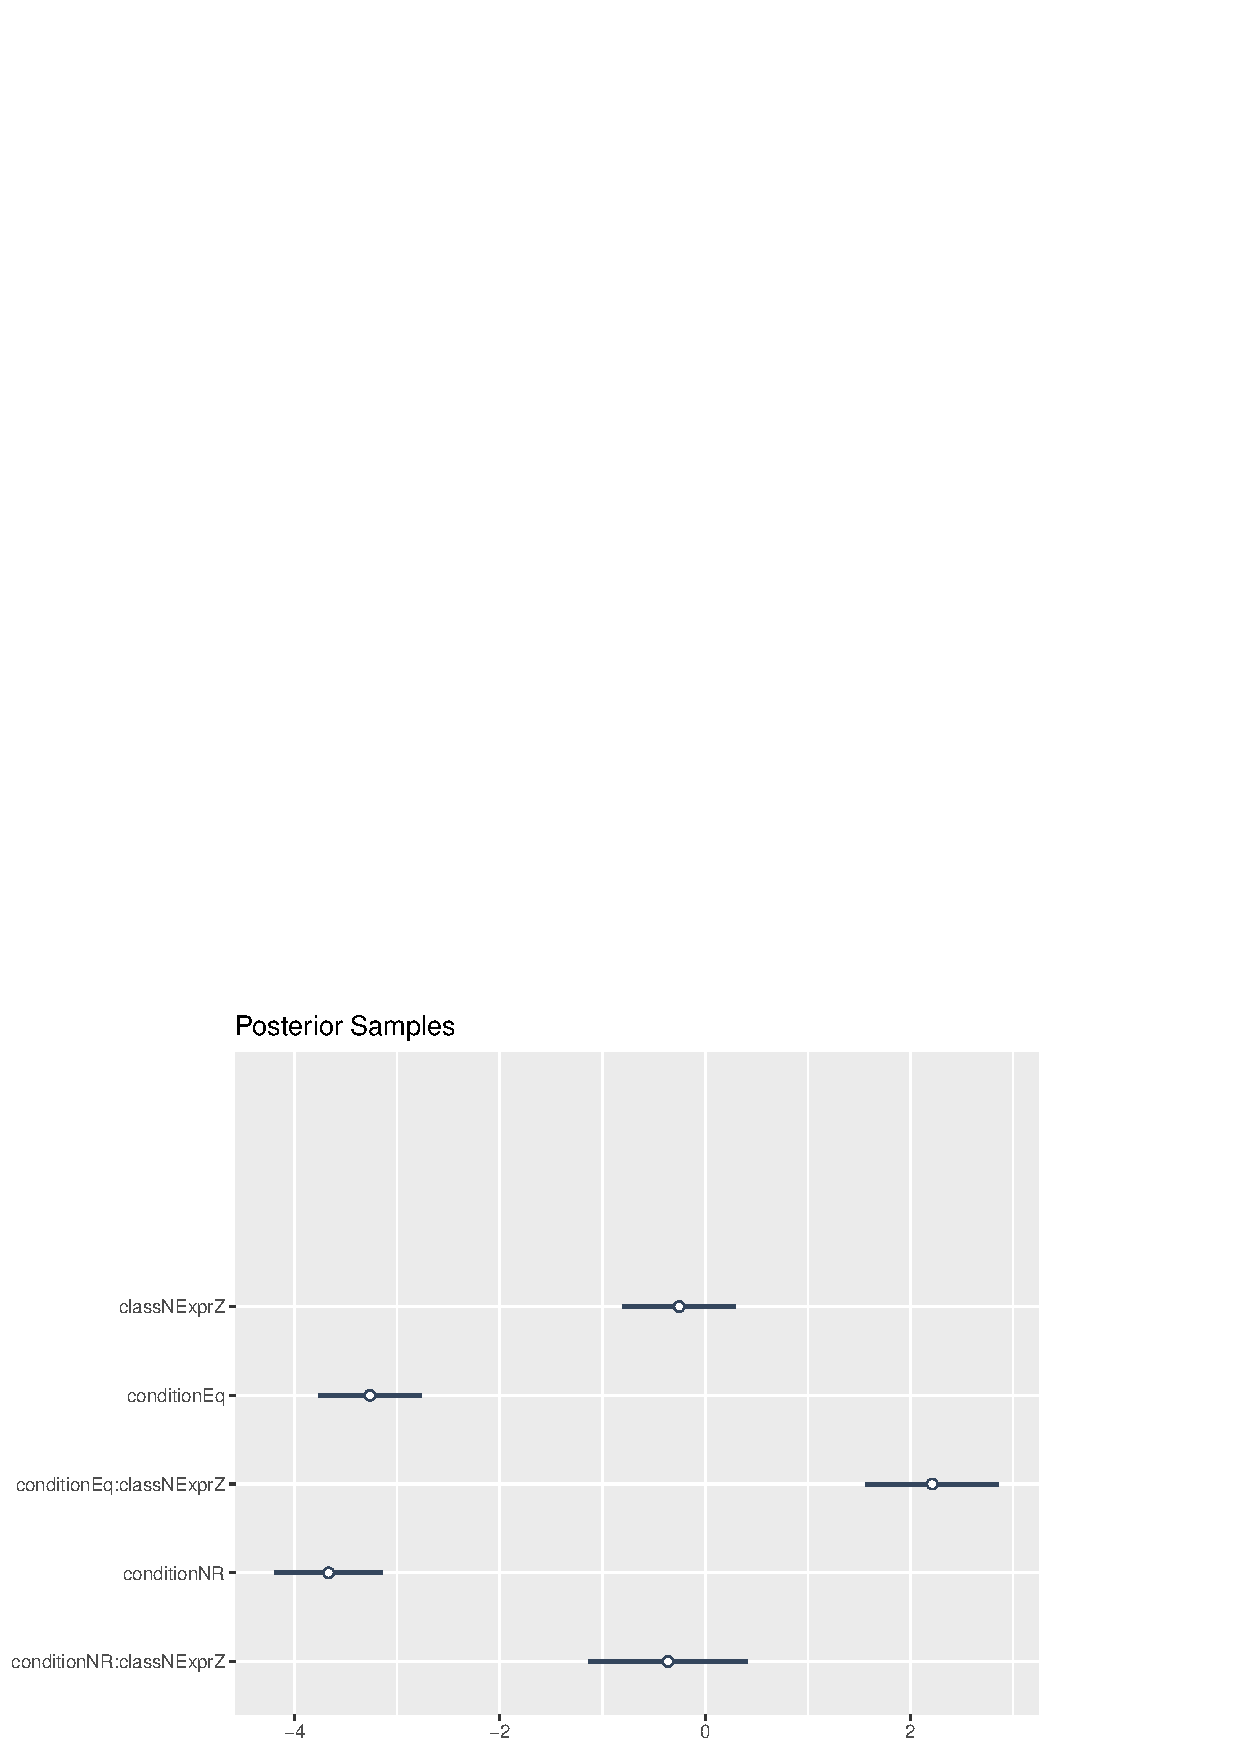
\includegraphics{posterior_graph.pdf}}

}

\caption{Graph of posterior samples}

\end{figure}
\end{frame}

\begin{frame}
\begin{enumerate}
\item
  main effects: all conditions were degraded against the baseline
\item
  \textbf{interaction effects}:
\end{enumerate}

\begin{itemize}
\tightlist
\item
  the strong positive effect of neg-words by equatives
\item
  weak negative interaction effect of neg-words by NegRaising
\item
  strong NPIs and neg-words not distinguishable in the baseline
\end{itemize}
\end{frame}

\begin{frame}[fragile]
\tiny

\begin{Shaded}
\begin{Highlighting}[]
\NormalTok{Summary of Posterior Distribution}

\NormalTok{Parameter               }\SpecialCharTok{|}\NormalTok{ Median }\SpecialCharTok{|}         \DecValTok{95}\SpecialCharTok{\% CI |     pd |          ROPE | \%} \ControlFlowTok{in}\NormalTok{ ROPE }\SpecialCharTok{|}\NormalTok{  Rhat }\SpecialCharTok{|}\NormalTok{     ESS}
\SpecialCharTok{{-}{-}{-}{-}{-}{-}{-}{-}{-}{-}{-}{-}{-}{-}{-}{-}{-}{-}{-}{-}{-}{-}{-}{-}{-}{-}{-}{-}{-}{-}{-}{-}{-}{-}{-}{-}{-}{-}{-}{-}{-}{-}{-}{-}{-}{-}{-}{-}{-}{-}{-}{-}{-}{-}{-}{-}{-}{-}{-}{-}{-}{-}{-}{-}{-}{-}{-}{-}{-}{-}{-}{-}{-}{-}{-}{-}{-}{-}{-}{-}{-}{-}{-}{-}{-}{-}{-}{-}{-}{-}{-}{-}{-}{-}{-}{-}{-}{-}{-}{-}{-}{-}{-}{-}}
\NormalTok{(Intercept)             }\SpecialCharTok{|}   \FloatTok{6.67} \SpecialCharTok{|}\NormalTok{ [ }\FloatTok{6.38}\NormalTok{,  }\FloatTok{6.95}\NormalTok{] }\SpecialCharTok{|}   \DecValTok{100}\SpecialCharTok{\% | [{-}0.10, 0.10] |        0\%} \ErrorTok{|} \FloatTok{1.002} \SpecialCharTok{|} \FloatTok{1905.00}
\NormalTok{conditionEq             }\SpecialCharTok{|}  \SpecialCharTok{{-}}\FloatTok{3.27} \SpecialCharTok{|}\NormalTok{ [}\SpecialCharTok{{-}}\FloatTok{3.53}\NormalTok{, }\SpecialCharTok{{-}}\FloatTok{3.00}\NormalTok{] }\SpecialCharTok{|}   \DecValTok{100}\SpecialCharTok{\% | [{-}0.10, 0.10] |        0\%} \ErrorTok{|} \FloatTok{1.000} \SpecialCharTok{|} \FloatTok{3381.00}
\NormalTok{conditionNR             }\SpecialCharTok{|}  \SpecialCharTok{{-}}\FloatTok{3.57} \SpecialCharTok{|}\NormalTok{ [}\SpecialCharTok{{-}}\FloatTok{3.86}\NormalTok{, }\SpecialCharTok{{-}}\FloatTok{3.30}\NormalTok{] }\SpecialCharTok{|}   \DecValTok{100}\SpecialCharTok{\% | [{-}0.10, 0.10] |        0\%} \ErrorTok{|} \FloatTok{1.000} \SpecialCharTok{|} \FloatTok{3320.00}
\NormalTok{classNExprZ             }\SpecialCharTok{|}  \SpecialCharTok{{-}}\FloatTok{0.20} \SpecialCharTok{|}\NormalTok{ [}\SpecialCharTok{{-}}\FloatTok{0.47}\NormalTok{,  }\FloatTok{0.08}\NormalTok{] }\SpecialCharTok{|} \FloatTok{92.30}\SpecialCharTok{\% | [{-}0.10, 0.10] |    23.08\%} \ErrorTok{|} \FloatTok{1.001} \SpecialCharTok{|} \FloatTok{2936.00}
\NormalTok{conditionEq}\SpecialCharTok{:}\NormalTok{classNExprZ }\SpecialCharTok{|}   \FloatTok{2.18} \SpecialCharTok{|}\NormalTok{ [ }\FloatTok{1.81}\NormalTok{,  }\FloatTok{2.58}\NormalTok{] }\SpecialCharTok{|}   \DecValTok{100}\SpecialCharTok{\% | [{-}0.10, 0.10] |        0\%} \ErrorTok{|} \FloatTok{1.002} \SpecialCharTok{|} \FloatTok{2954.00}
\NormalTok{conditionNR}\SpecialCharTok{:}\NormalTok{classNExprZ }\SpecialCharTok{|}  \SpecialCharTok{{-}}\FloatTok{0.53} \SpecialCharTok{|}\NormalTok{ [}\SpecialCharTok{{-}}\FloatTok{0.91}\NormalTok{, }\SpecialCharTok{{-}}\FloatTok{0.14}\NormalTok{] }\SpecialCharTok{|} \FloatTok{99.67}\SpecialCharTok{\% | [{-}0.10, 0.10] |        0\%} \ErrorTok{|} \FloatTok{1.001} \SpecialCharTok{|} \FloatTok{3027.00}
\end{Highlighting}
\end{Shaded}
\end{frame}

\begin{frame}
\begin{block}{How much variation is explained by the model?}
\protect\hypertarget{how-much-variation-is-explained-by-the-model}{}
\begin{itemize}
\tightlist
\item
  Bayesian models are not easily evaluated by the usual Multiple R or
  R-squared metrics
\item
  which represent how much variation in the dependend variable is
  explained by the model
\item
  but frequentist model with the same parameters reports:
\end{itemize}

Multiple R-squared: 0.5074, Adjusted R-squared: 0.5057

\begin{itemize}
\tightlist
\item
  see \href{data_analysis.html}{report}
\end{itemize}
\end{block}
\end{frame}

\begin{frame}
\begin{block}{Summary}
\protect\hypertarget{summary}{}
\begin{enumerate}
\tightlist
\item
  neg-words are (unlike strong NPIs) accepted in the standard of
  equatives
\end{enumerate}

\begin{itemize}
\tightlist
\item
  unexplainable in the syntactic theory of neg-words
\item
  NPI unacceptability is surprising but probably results from
  cross-linguistic differences in equatives
\end{itemize}

\begin{enumerate}
\setcounter{enumi}{1}
\item
  NegRaising predicates are better licensors for strong NPIs
\item
  in probability/scale manipulated contexts, strong NPIs are preferred
\end{enumerate}

\begin{itemize}
\tightlist
\item
  again problematic for the syntactic theory of neg-words
\end{itemize}

Intriguing correlations between conditions (per speaker).
\end{block}
\end{frame}

\begin{frame}
\begin{block}{Correlations}
\protect\hypertarget{correlations}{}
\begin{itemize}
\tightlist
\item
  all speakers agreed on their high acceptance of baseline
\item
  but some rated \emph{ani} high in equatives
\item
  but different group of speakers rated \emph{ani} high in NR (tables in
  the Appendix)
\item
  of the top ten speakers that rated \emph{ani} high in equatives, only
  1 rated \emph{ani} high in NR
\item
  similar observations in previous experiments: baselines universally
  accepted but divergent acceptability in non-baseline conditions
\end{itemize}
\end{block}
\end{frame}

\begin{frame}
\begin{block}{Correlations II}
\protect\hypertarget{correlations-ii}{}
\begin{itemize}
\tightlist
\item
  speakers who accept \emph{ani} in equatives treat it as neg-word
\item
  probably the result of the limited positive evidence to distinguish
  them: NegRaising, equatives, probability contexts
\item
  technically: there was no variation (or correlation with other
  conditions) with baseline -- uniform acceptability
\item
  z-transformation of (by subject) acceptance of conditions
\item
  checking the correlation of such z-transformed ratings
\item
  Pearson's product-moment correlation: t = \(-5.93\), p-value
  \(< 0.001\)
\end{itemize}
\end{block}
\end{frame}

\begin{frame}
\begin{figure}

{\centering \includegraphics{"correlations_ani.png"}

}

\caption{Correlations between NegRaising and Equatives}

\end{figure}
\end{frame}

\begin{frame}
\begin{itemize}
\tightlist
\item
  there are:
\end{itemize}

\begin{enumerate}
\item
  subjects who accept \emph{ani} with equatives but reject it with
  NegRaisers
\item
  subjects who accept \emph{ani} with NegRaisers but reject it with
  equatives
\end{enumerate}

The two sets don't intersect.

\begin{itemize}
\tightlist
\item
  this is a continuation of Dočekal and Dotlačil (2017): correlation
  between probability and NegRasing (for \emph{ani} but not for
  neg-words): see experiments below
\item
  but crucially, no correlations against the baseline: next slide
\item
  Pearson's product-moment correlation: t = \(-0.84\), p-value =
  \(0.41\)
\end{itemize}
\end{frame}

\begin{frame}
\begin{figure}

{\centering \includegraphics{"equatives_baseline_corr.png"}

}

\caption{Correlations between Equatives and Baseline}

\end{figure}
\end{frame}

\begin{frame}
\begin{block}{Distribution and correlations summary}
\protect\hypertarget{distribution-and-correlations-summary}{}
\begin{longtable}[]{@{}
  >{\raggedright\arraybackslash}p{(\columnwidth - 12\tabcolsep) * \real{0.2708}}
  >{\raggedright\arraybackslash}p{(\columnwidth - 12\tabcolsep) * \real{0.1042}}
  >{\raggedright\arraybackslash}p{(\columnwidth - 12\tabcolsep) * \real{0.1250}}
  >{\raggedright\arraybackslash}p{(\columnwidth - 12\tabcolsep) * \real{0.0833}}
  >{\raggedright\arraybackslash}p{(\columnwidth - 12\tabcolsep) * \real{0.0833}}
  >{\raggedright\arraybackslash}p{(\columnwidth - 12\tabcolsep) * \real{0.1458}}
  >{\raggedright\arraybackslash}p{(\columnwidth - 12\tabcolsep) * \real{0.1875}}@{}}
\toprule\noalign{}
\begin{minipage}[b]{\linewidth}\raggedright
\end{minipage} & \begin{minipage}[b]{\linewidth}\raggedright
Bas
\end{minipage} & \begin{minipage}[b]{\linewidth}\raggedright
Prob (unlik.)
\end{minipage} & \begin{minipage}[b]{\linewidth}\raggedright
Eq
\end{minipage} & \begin{minipage}[b]{\linewidth}\raggedright
NR
\end{minipage} & \begin{minipage}[b]{\linewidth}\raggedright
Fragm.
\end{minipage} & \begin{minipage}[b]{\linewidth}\raggedright
Without
\end{minipage} \\
\midrule\noalign{}
\endhead
strong NPIs & \(\checkmark\) & \(\checkmark\) & * & \(\checkmark\)* & *
& \(\checkmark\) \\
neg-words & \(\checkmark\) & * & \(\checkmark\) & * & \(\checkmark\)* &
\(\checkmark\) \\
\bottomrule\noalign{}
\end{longtable}

\begin{longtable}[]{@{}lllll@{}}
\toprule\noalign{}
& Eq \ldots{} NR & Prob. \ldots{} NR & Fragm. \ldots{} NR & Eq \ldots{}
Bas \\
\midrule\noalign{}
\endhead
strong NPIs & neg. corr. & neg. corr. & neg. corr. & * \\
neg-words & * & * & * & * \\
\bottomrule\noalign{}
\end{longtable}
\end{block}
\end{frame}

\begin{frame}{Theoretical consequences}
\protect\hypertarget{theoretical-consequences}{}
\begin{itemize}
\tightlist
\item
  general picture: both standard theories can explain the \textsc{bas}
  and \textsc{nr}
\item
  but only newer, alternative theory of negative concord can say
  something reasonable about neg-words acceptability in \textsc{eq}
\item
  and the semantic theory can give handle on speaker variation
\item
  skip to slide 60
\end{itemize}
\end{frame}

\begin{frame}
\begin{block}{Assumptions: licensing of (strong) NPIs}
\protect\hypertarget{assumptions-licensing-of-strong-npis}{}
\begin{itemize}
\tightlist
\item
  general framework: mixture of \emph{even}-theory of NPIs licensing
  (Krifka (1995),Lahiri (1998),Crnič (2014b) a.o.) and Gajewski's
  formalization of strong NPIs Jon R. Gajewski (2011)
\item
  licensing NPIs (after Jon R. Gajewski (2011)): strong NPIs are
  licensed in downward-entailing (DE) environments
\item
  DE both in Truth-Conditions (TC) but also in the non-at-issue meaning
\end{itemize}

\ex. An NPI is licensed in the environment \(\gamma\)\\
\([_\alpha exh [_\beta \ldots [_\gamma\) NPI \(] \ldots ]]\): \a. the
environment \(\gamma\) is DE in \(\beta\) \hfill weak NPIs \b. the
environment \(\gamma\) is DE in \(\alpha\) \hfill strong NPIs

~
\end{block}
\end{frame}

\begin{frame}
\begin{itemize}
\tightlist
\item
  the exhaustifier for strong NPIs as English \emph{even one}: covert
  \(even\)
\item
  the standard analysis for scalar strong NPIs Crnič (2014a) and for
  scalar reading of focus particles Panizza and Sudo (2020)
\item
  overt but also covert \emph{even} has scalar \Next[a] and additive
  \Next[b] presupposition:
\item
  the presuppositions after Panizza and Sudo (2020) (the additive
  sometimes suspended):
\end{itemize}

\ex. \a. Even Pope\(_F\) danced. \b. Even one\(_F\) cat will make Pope
happy.

\ex. `Even \(\phi\)' presupposes: \a. that \(\phi\) is relatively
unlikely to be true among Alt(\(\phi\)); and \b. that there is
\(\psi \in\) Alt(\(\phi\)) that is not entailed by \(\phi\) and is true.

\footnotesize(for monotonic scales, likelihood translates into
entailment (after Crnič (2011)\}))\normalsize
\end{frame}

\begin{frame}
\begin{block}{Baseline from the experiment}
\protect\hypertarget{baseline-from-the-experiment}{}
\begin{itemize}
\tightlist
\item
  \emph{ani} strong NPIs associate with covert \emph{even} (scope:
  propositional level)
\item
  it reqires DE both in TC and non-at-issue
\item
  plus the scalar presupposition of covert \emph{even} exhaustifier
\item
  the exhaustified focus alternatives: other cardinality predicates
  (after Lahiri (1998),Crnič (2011) a.o.)
\end{itemize}
\end{block}
\end{frame}

\begin{frame}
\begin{itemize}
\tightlist
\item
  the entailment between numerals is reversed by negation:
  \(\neg (\llbracket\) one cat
  \(\rrbracket \ldots) \models \neg(\llbracket\)two
  cats\(\rrbracket \ldots)\)
\end{itemize}

\ex. Ani one thief neg-remained in the kingdom.\\
\a. ~{[}\(_\alpha\) (\(even\)) {[}\(_\beta\)
\neg [$_\gamma$ ani one thief remained in the kingdom ]{]} {]} \a. TC
(in \(\beta\)) DE: \(\checkmark\) \b. non-at-issue (in \(\alpha\)) DE:
\(\checkmark\) \c. scalar presupposition of (even): \(\rightarrow\)
\(\neg\)(two thieves remained), \(\neg\)(three thieves remained),
\ldots: \(\checkmark\) \d. additive presupposition: \(\neg\)(two thieves
remained) \(\vee\) \(\neg\)(three thieves remained), \ldots:
\(\checkmark\) \z.

~
\end{frame}

\begin{frame}
\begin{block}{Other conditions from the experiment}
\protect\hypertarget{other-conditions-from-the-experiment}{}
\begin{block}{Likelihood}
\protect\hypertarget{likelihood}{}
\begin{itemize}
\tightlist
\item
  for \textsc{bottom}: the explanation is the same as for the baseline
\item
  the scope (\(even\)) \textgreater{} \(\neg\) \textgreater{} \ldots{}
  one \ldots{}
\item
  the general preference of strong NPIs over neg-words follows from the
  semantic theory of neg-words

  \begin{itemize}
  \tightlist
  \item
    core idea: neg-words presuppose emptiness of their discourse
    referent extension
  \end{itemize}
\item
  all the items were (nearly always) constructed in such a way that
  there was a positive inference (some diamonds were found, etc.: )
\end{itemize}
\end{block}
\end{block}
\end{frame}

\begin{frame}
\begin{block}{Neg-Raising}
\protect\hypertarget{neg-raising}{}
\begin{itemize}
\tightlist
\item
  in many previous experiments (three at least): Neg-Raising was better
  accepted with strong NPIs
\item
  but the effect was never strong; in the last two the effect
  disappeared
\item
  one possibility: the variation -- speakers who treat \emph{ani} as a
  neg-word blur the line
\item
  standard theories of Neg-Raising: Jon Robert Gajewski (2007) or Romoli
  (2013)
\item
  the scope of negation (via the excluded middle inference) on the
  embedded predicate
\item
  at the embedded level: covert (\(even\)) \textgreater{} \(\neg\)
  \textgreater{} {[}\ldots{} one \ldots{]}
\item
  neg-words: the locality constraints -- see below
\item
  Equatives: more in the neg-words section
\end{itemize}
\end{block}
\end{frame}

\begin{frame}
\begin{block}{Neg-words}
\protect\hypertarget{neg-words-1}{}
\begin{itemize}
\tightlist
\item
  semantic/pragmatic theory of neg-words and negative concord
\item
  Ovalle and Guerzoni (2004) and modern reformulation in Kuhn (2022)
\item
  TC: indefinite description
\item
  non-at-issue: empty reference
\end{itemize}

\ex. \a.
\(\llbracket\)neg-word\(\rrbracket\)=\(\lambda P.\exists x[SORT(x) \wedge P(x)]\)
\hfill TC \b.
\(\llbracket\)neg-word\(\rrbracket\)=\(\neg \exists x[SORT(x) \wedge P(x)]\)
\hfill non-at-issue \a. after Kuhn (2022): \(\wedge \mathbf{0_x}\)
\ldots postsupposition (highest scope) \z.

~
\end{block}
\end{frame}

\begin{frame}
\begin{block}{Locality, etc.}
\protect\hypertarget{locality-etc.}{}
\begin{itemize}
\tightlist
\item
  Kuhn (2022): many improvements of Ovalle and Guerzoni (2004)
\item
  discourse referents (presupposed to be empty) are delimited by the
  previous context

  \begin{itemize}
  \tightlist
  \item
    more specific concerning the presupposition of emptiness
  \end{itemize}
\item
  neg-words are analyzed via split scope around licensor (prototypically
  negation)

  \begin{itemize}
  \tightlist
  \item
    the split scope is achieved via quantifier raising
  \item
    the locality constraints on neg-word licensing \(\approx\) QR in the
    particular language and construction
  \end{itemize}
\end{itemize}
\end{block}
\end{frame}

\begin{frame}
\begin{block}{Explaining the baseline}
\protect\hypertarget{explaining-the-baseline}{}
\ex. neg-word thief neg-remained in the kingdom. \a.
{[}\(\neg[\exists x[\mathbf{thief}(x) \wedge \mathbf{remained}(x)]\)
{]}{]} \(\wedge \mathbf{0_x}\)

\begin{itemize}
\tightlist
\item
  TC and the postsupposition are compatible
\item
  in positive sentences, the \(\mathbf{0_x}\) postsupposition leads to
  ungrammaticality:
\end{itemize}

\ex. neg-word thief remained in the kingdom. \a.
{[}\(\exists x[\mathbf{thief}(x) \wedge \mathbf{remained}(x)]\) {]}
\(\wedge \mathbf{0_x}\) \hfill \(\bot\)

\begin{itemize}
\tightlist
\item
  this also nicely explains the acceptability of neg-words with
  \emph{bez} `without' (no morphological negation)
\end{itemize}
\end{block}
\end{frame}

\begin{frame}
\begin{block}{Other conditions from the experiment}
\protect\hypertarget{other-conditions-from-the-experiment-1}{}
\begin{block}{Probability}
\protect\hypertarget{probability}{}
\begin{itemize}
\tightlist
\item
  both in top and bottom contexts, strong NPIs were preferred
\item
  the contexts were (nearly always) set up with positive inference
\item
  the positive inference goes against \(\mathbf{0_x}\) presupposition of
  neg-words

  \begin{itemize}
  \tightlist
  \item
    it can also explain the surprisingly high acceptability of strong
    NPIs even in top scalar contexts
  \item
    another factor: different scales (numerical in last experiment,
    ad-hoc in previous) \(\rightarrow\) future experimental work
  \end{itemize}
\end{itemize}
\end{block}
\end{block}
\end{frame}

\begin{frame}
\begin{block}{Neg-Raising}
\protect\hypertarget{neg-raising-1}{}
\begin{itemize}
\tightlist
\item
  previous experimental work: mostly evidence for decreased
  acceptability of neg-words (against strong NPIs) in NR
\item
  Kuhn's QR approach: explains the neg-words decreased acceptability
\item
  in the last experiment: the contrast is blurred
\item
  one possibility: to remove subjects treating \emph{ani} as a neg-word
  from the stats
\item
  unlike with equatives, the environment seems to be nearly as
  acceptable for neg-words as for strong NPIs
\end{itemize}
\end{block}
\end{frame}

\begin{frame}
\begin{block}{Equatives}
\protect\hypertarget{equatives}{}
\begin{itemize}
\tightlist
\item
  Slavic equatives are different from English equatives, and their
  morpho-syntax is very similar to correlatives

  \begin{itemize}
  \tightlist
  \item
    Slavic equatives are built on the correlative syntax
  \item
    and following Jacobson (1995): correlatives are bad licensors of
    NPIs
  \end{itemize}
\item
  another experiment in preparation: weak NPIs are penalized in Czech
  equatives (but acceptable in comparatives)

  \begin{itemize}
  \tightlist
  \item
    Slavic equatives are probably not even DE (as was observed for
    German: Krifka (1992),Penka (2016))
  \end{itemize}
\item
  neg-words are acceptable but verbal negation not (as in German: Penka
  (2016))
\end{itemize}

\exg. Petr je tak chytrý jak nikdo jiný/*Marie ne.\\
Petr is so smart how neg-word else/Mary not\\
\hspace*{0.333em}

~
\end{block}
\end{frame}

\begin{frame}
\begin{block}{Equatives II}
\protect\hypertarget{equatives-ii}{}
\begin{itemize}
\tightlist
\item
  syntactic and semantic ingredients (pseudoCzech in \Next)
\item
  non-standard: \(max \rightarrow max_{inf}\) (otherwise \(max\) would
  lead to \(\bot\)): Penka (2016)
\end{itemize}

\ex. This thief is so clever how neg-word other thief.\\
\a. {[} so {[}so\(_1\) no other thief \(t_1\) clever {]}{]}\(_2\)
{[}This thief is \(t_2\) clever{]}\\
\b. \(\llbracket so\rrbracket\) \ldots{} picks up the degree denoted by
the standard clause\\
\b. \(\llbracket\) how\(_1\) neg-word other thief clever is
\(\rrbracket\)\\
\a. nobody other than the thief is \(d\)-clever \hfill neg-word
presupposition\\
\b. the thief is \(d\)-clever \hfill implicature of \emph{other}\\
\z.

\ex. \a. \(\llbracket\) as
\(\rrbracket = \lambda S\lambda C.max(C) \geq max(S)\)\\
\b.
\(S' \subseteq S: max(C) \geq max(S) \rightarrow max(C) \geq max(S')\)
\hfill English DE \textit{as}

~
\end{block}
\end{frame}

\begin{frame}
\begin{block}{Equatives III}
\protect\hypertarget{equatives-iii}{}
Motivation of the ingredients:

\begin{itemize}
\tightlist
\item
  \(max_{inf}\): the equative in Czech has exactly the same building
  blocks (\emph{tak} `so' \ldots{} \emph{jak} `how') as correlative
  constructions
\item
  \emph{other}: the anaphor similar to reciprocal anaphors

  \begin{itemize}
  \tightlist
  \item
    it identifies the dref
  \item
    it is also used in the exceptive phrases from which the
    presupposition comes: \emph{Nobody other than John neg-came}
    presupposes that John came (as the only exception)
  \end{itemize}
\item
  neg-word presupposition ranges over the dref picked up by the
  reciprocal
\end{itemize}
\end{block}
\end{frame}

\begin{frame}
\begin{block}{Summary 1}
\protect\hypertarget{summary-1}{}
\begin{itemize}
\tightlist
\item
  Czech neg-words and strong NPIs
\item
  existential TC core: \(\lambda P.\exists x[NP(x) \wedge P(x)]\)
\end{itemize}

\begin{longtable}[]{@{}lll@{}}
\toprule\noalign{}
& TC & non-at-issue meaning \\
\midrule\noalign{}
\endhead
neg-words & existential & \(\mathbf{0_x}\) \\
strong NPIs & existential & scalar presupposition \\
& & association with (even) \\
\bottomrule\noalign{}
\end{longtable}
\end{block}
\end{frame}

\begin{frame}
\begin{itemize}
\tightlist
\item
  that explains (with some other more or less standard assumptions) the
  patterns of the experiment(s)
\item
  the answer to Question 1 :
\end{itemize}

\ex. Question1: \a. How can we explain microvariation by grammatical
(semantic) factors? \b. Is part of the variation caused by social
factors? \z.

\ex. The speaker variation is explainable as shifting from the scalar to
the emptiness of the DR presupposition (in case of \emph{ani jeden}
`even one'). \a. Social factors don't seem to play a role in this shift.

~
\end{frame}

\begin{frame}
\begin{itemize}
\tightlist
\item
  the experimental data support the semantic theory of neg-words
\item
  obvious problems for the syntactic approach:

  \begin{itemize}
  \tightlist
  \item
    neg-words in equatives: no standard theory of equatives with
    interpreted \(\neg\) ({[}uNeg{]}) in the standard
  \item
    higher acceptability of strong NPIs in the probability manipulated
    contexts: unpredicted
  \item
    non-stipulative explanation for fragmentary answers preference for
    neg-words and also \emph{without} type of P
  \end{itemize}
\end{itemize}
\end{frame}

\begin{frame}
\begin{block}{Summary 2}
\protect\hypertarget{summary-2}{}
\ex. How to explain the unpredicted acceptability of neg-words in
equatives (and NPIs unavailability)?

\ex. The non-standard \(max_{inf}\) accounts for the surprising
neg-words acceptability.\\
\a. decisive evidence for the semantic theory of neg-words\\
\b. non-monotonic environment: NPIs are predicted to be out

\begin{itemize}
\tightlist
\item
  prediction: minimizers (and other non-monotonic tolerating) NPIs
  should be ok \ldots{} intuitively correct
\end{itemize}
\end{block}
\end{frame}

\begin{frame}
\begin{center}
\Huge Thanks!
\end{center}

\normalsize
\end{frame}

\begin{frame}
\begin{block}{Open questions}
\protect\hypertarget{open-questions}{}
\begin{itemize}
\tightlist
\item
  proper investigation of locality constraints

  \begin{itemize}
  \tightlist
  \item
    NegRaising: the concurrence sometimes vanishes (Maximize
    Presupposition of Heim (1991)?)
  \end{itemize}
\item
  both scopes of covert \emph{even} in probability contexts (exp1) or
  just one (exp2 \& exp3), or the difference comes from different
  scales?
\item
  cross-linguistic variation in the neg-words locality: at least in some
  Romance languages, neg-words are licensed in \emph{before}-clauses and
  under \emph{doubt}-type of predicates

  \begin{itemize}
  \tightlist
  \item
    some suggestions in Kuhn (2022)
  \end{itemize}
\end{itemize}
\end{block}
\end{frame}

\begin{frame}{Appendix}
\protect\hypertarget{appendix}{}
\begin{block}{Histograms}
\protect\hypertarget{histograms}{}
\begin{figure}

{\centering \includegraphics{"histogram_faceted_prob_bott.png"}

}

\caption{Histogram: probabilities Bottom of the scale}

\end{figure}
\end{block}
\end{frame}

\begin{frame}
\begin{figure}

{\centering \includegraphics{"histogram_faceted_prob_top.png"}

}

\caption{Histogram: probabilities Top of the scale}

\end{figure}
\end{frame}

\begin{frame}
\begin{block}{Items}
\protect\hypertarget{items}{}
\begin{itemize}
\tightlist
\item
  the predicates in baseline and NegRaising conditions were the same
\item
  with equatives, this wasn't possible to realize, but the sentences
  were constructed as close to the meaning of baseline and NegRaising as
  possible
\item
  and the standard of equatives was always the same neg-word NP/strong
  NPI as in the baseline and NegRaising conditions
\end{itemize}
\end{block}
\end{frame}

\begin{frame}
\end{frame}

\begin{frame}
\begin{block}{Demographic factors II}
\protect\hypertarget{demographic-factors-ii}{}
\begin{enumerate}
\tightlist
\item
  region:
\end{enumerate}

\begin{itemize}
\tightlist
\item
  all regions of the Czech Republic aggregated to Bohemia vs.~Moravia:
\item
  67\% of subjects were from Bohemia, 33\% from Moravia
\item
  no significant main or interaction effect was found
\end{itemize}

\begin{enumerate}
\setcounter{enumi}{1}
\tightlist
\item
  age:
\end{enumerate}

\begin{itemize}
\tightlist
\item
  range: 19 to 71 years, mean: 25.6, median: 23
\item
  only significant interaction effect: younger people (under 27) rated
  probability condition slightly better (t-value: \(2.02\), p
  \(< 0.05\))
\end{itemize}
\end{block}
\end{frame}

\begin{frame}
\begin{block}{Demographic factors III}
\protect\hypertarget{demographic-factors-iii}{}
\begin{enumerate}
\setcounter{enumi}{2}
\tightlist
\item
  reading time
\end{enumerate}

\begin{itemize}
\tightlist
\item
  a proxy for education bias
\item
  reading time of books and other media: 0 to 10 hours
\item
  mean: 1.43, median: 1 hour
\item
  only one significant interaction: subjects with reading time
  \textgreater{} 1 hour rated NR-condition better (t-value \(2.05\), p
  \(< 0.05\))
\end{itemize}
\end{block}
\end{frame}

\begin{frame}
\begin{block}{More models}
\protect\hypertarget{more-models}{}
\begin{itemize}
\tightlist
\item
  Bayesian model for experiment 1: next slide
\item
  confidence intervals agree with p-values from the cumulative mixed
  model
\end{itemize}
\end{block}
\end{frame}

\begin{frame}
\begin{figure}

{\centering \includegraphics{"acc-results-complex.png"}

}

\caption{Bayesian model}

\end{figure}
\end{frame}

\begin{frame}
\begin{itemize}
\tightlist
\item
  mixed linear model for the top of the scale (probability)
\end{itemize}

\footnotesize
\end{frame}

\begin{frame}
\begin{itemize}
\tightlist
\item
  the last experiment: surprisingly high acceptability of strong NPIs in
  the top of the scale contexts
\item
  in previous experiments, we tested top of the scale, and neg-words
  were better accepted
\item
  one possible explanation: the nature of the scale:

  \begin{itemize}
  \tightlist
  \item
    the last experiment: just numerical scales, the two before social
    hierarchies, not numerical scales
  \end{itemize}
\item
  future experiment: probabilities and different scales
\end{itemize}
\end{frame}

\begin{frame}
\begin{block}{Strong negative effect of neg-words}
\protect\hypertarget{strong-negative-effect-of-neg-words}{}
\begin{itemize}
\tightlist
\item
  not as strong as the conditions
\item
  unclear reason
\item
  but it is not frequency:
\item
  Czech National Corpus Křen et al. (2015) search for \emph{ani} plus
  numeral, noun, pronoun, preposition
\item
  the same for \emph{žádný} and the same categories: \Next
\item
  their frequency is nearly the same
\end{itemize}

\ex. \a. {[}ani \ldots{]}: 73 917 hits \b. {[}žádný \ldots{]}: 66 912

~
\end{block}
\end{frame}

\begin{frame}
\begin{itemize}
\tightlist
\item
  possible syntactic factor: first query into Křen et al. (2015)
\item
  asymmetry between \emph{ani} and \emph{žádný} in terms of their scope
  preferences
\item
  \emph{žádný} preferentially scopes in VP
\item
  Burnett, Koopman, and Tagliamonte (2018): the distinction between
  negative indefinites and NPIs (hard constraint in Scandinavian, soft
  constraint in English)

  \begin{itemize}
  \tightlist
  \item
    handle for: neg-words do have syntactic component, NPIs not
  \end{itemize}
\item
  3 out of 4 conditions in the experiment: strong NPI/neg-word in
  subject
\end{itemize}

\ex. \a. žádný `no': \a. 11 580 in Subj, 19 445 in Obj \z. \b. ani
`even' \a. 8 661 in Subj, 8 562 in Obj \z.

~
\end{frame}

\begin{frame}
\begin{block}{The correlation table (subjects)}
\protect\hypertarget{the-correlation-table-subjects}{}
\tiny
\end{block}
\end{frame}

\begin{frame}
\begin{block}{Historical note (Czech)}
\protect\hypertarget{historical-note-czech}{}
\begin{itemize}
\tightlist
\item
  diachronic linguists (Bauer, Lamprecht, and Šlosar (1986),Holub and
  Kopečný (1952)): at least some neg-words are newer than strong NPIs:
\item
  neg-words (because appearing in negative clauses frequently) acquired
  the modern \emph{no} meaning
\item
  strong NPIs are older
\end{itemize}
\end{block}
\end{frame}

\begin{frame}
\begin{block}{Old Czech data}
\protect\hypertarget{old-czech-data}{}
\begin{itemize}
\tightlist
\item
  strong NPIs are older than neg-words: \emph{ani jeden hrad neg-V} from
  14\(^{\textrm{th}}\) century
\end{itemize}

\exg. Dám tobě zemi žádnú.\\
give.\textsc{1sg} to-you land wanted\\
`I will give you the wanted land.' \hfill old Czech

\exg. Nedám ti žádnou zemi.\\
give.\textsc{1sg} to-you no land\\
`I will give you no land.' \hfill modern Czech

~

\begin{longtable}[]{@{}
  >{\raggedright\arraybackslash}p{(\columnwidth - 0\tabcolsep) * \real{0.0556}}@{}}
\toprule\noalign{}
\endhead
\#\# Experiment 2 \\
- the previous results are no outliers - similar correlations were
obtained in two other experiments - Experiment 2 \\
- 40 Czech native speakers (students of MUNI) - again, mostly
acceptability judgment task (Likert scale 1..5) - but also truth value
judgment task (likelihood condition) \\
\bottomrule\noalign{}
\end{longtable}

\begin{block}{Experiment 2 example item}
\protect\hypertarget{experiment-2-example-item}{}
\ex. \cond{BASELINE} \ag. A: Koho vyhodil professor Palný včera ze
zkoušky?\\
A: whom failed professor Palny yesterday from exam\\
`Who was failed by professor Palny during yesterday's exam?' \bg. B:
Profesor ne-vyhodil (POLARITY-ITEM) studenta.\\
B: professor NEG-failed POLARITY-ITEM student\\
`Anyone/even one student wasn't failed by the professor.'

~
\end{block}
\end{block}
\end{frame}

\begin{frame}
\ex. \cond{ELLIPSIS} \ag. A: Koho vyhodil professor Palný včera ze
zkoušky?\\
A: whom failed professor Palny yesterday from exam\\
`Who was failed by professor Palny during yesterday's exam?' \bg. B:
(POLARITY-ITEM) studenta.\\
B: POLARITY-ITEM student\\
`Not any /Not even one student.'

~
\end{frame}

\begin{frame}
\ex. \cond{NR} \ag. A: Co je nového na katedrových zkouškách?\\
A: what is new at department exams\\
`What happened new during the department exams?' \bg. Profesor Palný
nechce, abychom vyhodili (POLARITY-ITEM) studenta\\
professor Palny neg-wants COMP fail POLARITY-ITEM student\\
`Professor Palny doesn't want any/even one student to fail.'

~
\end{frame}

\begin{frame}
\ex. \cond{LIKELIHOOD} \a. Yesterday, Professor Novák ran exams of a
fairly easy lecture, which is attended by bachelors, masters and
doctoral students. Doctoral students always pass the exam, masters
usually do, bachelors rather don't.' \bg. Včerejší zkoušku u prof.
Nováka nesložili (POLARITY-ITEM) bakaláři.\\
yesterday exam by professor Novak neg-passed POLARITY-ITEM bachelors\\
`Any/even bachelors didn't pass professor Novak's exam yesterday.'

\begin{itemize}
\tightlist
\item
  notice: the likelihood of context is reversed -- \emph{ani} is
  expected to fare worse
\end{itemize}
\end{frame}

\begin{frame}
\begin{itemize}
\tightlist
\item
  the experiment was a 4x2 design
\item
  the descriptive summary follows
\item
  the main effects are all significantly negative against the baseline
\end{itemize}

\begin{enumerate}
\item
  in \cond{LIKELIHOOD} strong positive interaction effect by
  \emph{žádný}: t-value = \(8.32\)
\item
  no significant interaction effect of \cond{ELLIPSIS} by the
  expression: the context seems to meliorate the difference between
  strong NPIs and neg-words
\item
  the interaction between \cond{NR} and the expression is nearly
  significant
\end{enumerate}
\end{frame}

\begin{frame}
\begin{figure}

{\centering \includegraphics{"error_bar_exp_2.png"}

}

\caption{Graph of acceptance (+error bars) Experiment 2}

\end{figure}
\end{frame}

\begin{frame}
\begin{block}{Correlations in Experiment 2}
\protect\hypertarget{correlations-in-experiment-2}{}
\begin{itemize}
\tightlist
\item
  again, the correlation between the type of expression and its
  acceptability in tested environments was searched
\end{itemize}

\begin{enumerate}
\tightlist
\item
  strong and highly significant negative correlation between
  \cond{LIKELIHOOD} and \cond{NR}: t-value = \(−3.2\) p=\(.003\)
\end{enumerate}

\begin{itemize}
\tightlist
\item
  see the figure on the next slide; again z-transformation
\end{itemize}

\begin{enumerate}
\setcounter{enumi}{1}
\tightlist
\item
  significant correlation between \cond{ELLIPSIS} and NR-responses with
  \emph{ani}: t-value = \(−2.1\), p = \(.04\)
\end{enumerate}
\end{block}
\end{frame}

\begin{frame}
\begin{figure}

{\centering \includegraphics{"exp2_correlations_ani.png"}

}

\caption{Correlation between LIKELIHOOD and NR (ani) Experiment 2}

\end{figure}
\end{frame}

\begin{frame}
As for the correlations between \emph{žádný} and
\cond{ELLIPSIS}/\cond{NR} or \cond{LIKELIHOOD}/\cond{NR}

\begin{itemize}
\tightlist
\item
  the expectation is to find no correlation
\item
  and indeed: all models: p \textgreater{} \(.1\)

  \begin{itemize}
  \tightlist
  \item
    \cond{LIKELIHOOD} and \cond{NR} with respect to \emph{žádný}:
    negative but not significant (t = \(–1.6\), p = \(0.11\)) unlike for
    \(ani\)
  \item
    see the figure on the next slide
  \end{itemize}
\end{itemize}
\end{frame}

\begin{frame}
\begin{figure}

{\centering \includegraphics{"exp2_correlation_zadny.png"}

}

\caption{Correlation between LIKELIHOOD and NR (žádný) Experiment 2}

\end{figure}
\end{frame}

\begin{frame}
\begin{block}{Experiment 3}
\protect\hypertarget{experiment-3}{}
\begin{itemize}
\tightlist
\item
  very similar design as experiment 2 (previous version)
\item
  five conditions against crossed with the polarity-item: 5x2:
\item
  25 items, 25 fillers
\end{itemize}

\begin{enumerate}
\item
  \cond{NR}
\item
  \cond{ELLIPSIS}
\item
  \cond{WITHOUT}
\item
  \cond{LIKELIHOOD}
\item
  \cond{IDIOM}
\end{enumerate}
\end{block}
\end{frame}

\begin{frame}
\begin{itemize}
\tightlist
\item
  55 participants, one excluded for a bad score in fillers
\item
  mostly students of MUNI in Brno
\item
  examples of \cond{WITHOUT} and \cond{LIKELIHOOD}:
\item
  the error bar graph in Figure 10
\end{itemize}
\end{frame}

\begin{frame}
\ex. \cond{WITHOUT} \ag. Prodal mu dvě šachové sady bez (POLARITY-ITEM)
krále.\\
sold him two chess sets without POLARITY-ITEM king\\
`He sold him two chess sets without any/even one king'

\begin{itemize}
\tightlist
\item
  notice: Czech \emph{bez} doesn't bear any morphological negation
\end{itemize}
\end{frame}

\begin{frame}
\ex. \cond{LIKELIHOOD} \ag. Ten kněz byl cílevědomý, ale neschopný,
takže se nestal (POLARITY-ITEM) kardinálem.\\
The priest was purposeful but incompetent therefore SE NEG-became
POLARITY-ITEM cardinal\\
`The priest was purposeful but incompetent; therefore, he didn't become
any/even cardinal.'

\begin{itemize}
\tightlist
\item
  notice: as in experiment 2, the context likelihood goes against the
  \emph{even} presupposition of \emph{ani}
\end{itemize}
\end{frame}

\begin{frame}
\begin{figure}

{\centering \includegraphics{"error_bar_exp3.png"}

}

\caption{Graph of acceptance (+error bars) Experiment 3}

\end{figure}
\end{frame}

\begin{frame}
\begin{itemize}
\tightlist
\item
  again mixed-models
\item
  \cond{WITHOUT}: baseline -- both polarity items were indistinguishable
  in the baseline
\item
  three important interaction effects:
\end{itemize}

\begin{enumerate}
\item
  \emph{ani} was considered worse in \cond{ELLIPSIS}: t = \(-2.61\), p
  \(<.01\)
\item
  \emph{ani} was worse in \cond{LIKELIHOOD}: t = \(-4.73\), p \(<.001\)
\item
  \emph{ani} was better in \cond{NR}: t = \(2.41\), p \(<.05\) (similar
  findings as in older experimental work focused on NegRaising: Dočekal
  and Dotlačil (2016a),Dočekal and Dotlačil (2016b))
\end{enumerate}
\end{frame}

\begin{frame}
\begin{itemize}
\tightlist
\item
  the baseline shows that both polarity items can appear in sentences
  without verbal negation
\item
  the positive interaction of \emph{ani} by \cond{ELLIPSIS}: expected
  for NPIs
\item
  in both experiment 2 and experiment 3 \emph{ani} was tested in
  \cond{LIKELIHOOD} with a bad probability/noteworthiness profile for it

  \begin{itemize}
  \tightlist
  \item
    but the scales were ranks (nouns), not numerical
  \item
    in both experiments, \emph{ani} was judged as worse in
    \cond{LIKELIHOOD} than \emph{žádný}
  \end{itemize}
\end{itemize}
\end{frame}

\begin{frame}
\begin{block}{The correlation in experiment 3 and summary}
\protect\hypertarget{the-correlation-in-experiment-3-and-summary}{}
\begin{itemize}
\tightlist
\item
  again, the negative correlation between \emph{ani} acceptability in
  \cond{NR} and its acceptability in \cond{LIKELIHOOD} was found
\item
  t=\(-3.0\), p \(<0.005\)
\end{itemize}
\end{block}
\end{frame}

\begin{frame}
\begin{itemize}
\tightlist
\item
  in all three experiments, the following negative correlations for
  \emph{ani} were found:
\end{itemize}

\begin{enumerate}
\item
  the acceptability in \cond{EQUATIVES} and \emph{ani} acceptability in
  \cond{NR} (experiment 1)
\item
  the acceptability in \cond{LIKELIHOOD} and \emph{ani} acceptability in
  \cond{NR} (experiment 2 \& 3)
\item
  the acceptability in \cond{ELLIPSIS} and \emph{ani} acceptability in
  \cond{NR} (experiment 2)
\end{enumerate}
\end{frame}

\begin{frame}
\end{frame}

\begin{frame}{References}
\protect\hypertarget{references}{}
\hypertarget{refs}{}
\begin{CSLReferences}{1}{0}
\leavevmode\vadjust pre{\hypertarget{ref-alexandropoulou2020there}{}}%
Alexandropoulou, Stavroula, Lisa Bylinina, and Rick Nouwen. 2020. {``Is
There \emph{Any} Licensing in Non-{DE} Contexts? {A}n Experimental
Study.''} In \emph{Proceedings of Sinn Und Bedeutung}, edited by M.
Franke et al., 24:35--47. 1.

\leavevmode\vadjust pre{\hypertarget{ref-Bauer:1986}{}}%
Bauer, J., A. Lamprecht, and D. Šlosar. 1986. \emph{Historická Mluvnice
Češtiny}. SPN.

\leavevmode\vadjust pre{\hypertarget{ref-beck201913}{}}%
Beck, Sigrid. 2019. {``13 Comparison Constructions.''}
\emph{Semantics-Lexical Structures and Adjectives}, 415.

\leavevmode\vadjust pre{\hypertarget{ref-burnett2018structural}{}}%
Burnett, Heather, Hilda Koopman, and Sali A Tagliamonte. 2018.
{``Structural Explanations in Syntactic Variation: The Evolution of
English Negative and Polarity Indefinites.''} \emph{Language Variation
and Change} 30 (1): 83--107.

\leavevmode\vadjust pre{\hypertarget{ref-burnett2015variable}{}}%
Burnett, Heather, Mireille Tremblay, and Hélène Blondeau. 2015. {``The
Variable Grammar of Negative Concord in Montr{é}al French.''}
\emph{University of Pennsylvania Working Papers in Linguistics} 21 (2):
3.

\leavevmode\vadjust pre{\hypertarget{ref-Chemla-Homer-Rothschild-NPI}{}}%
Chemla, Emmanuel, Vincent Homer, and Daniel Rothschild. 2011.
{``Modularity and Intuitions in Formal Semantics: The Case of Polarity
Items.''} \emph{Linguistics and Philosophy} 34 (6): 537--70.
\url{https://doi.org/10.1007/s10988-012-9106-0}.

\leavevmode\vadjust pre{\hypertarget{ref-chierchia2019factivity}{}}%
Chierchia, Gennaro. 2019. {``Factivity Meets Polarity: On Two
Differences Between {I}talian Versus {E}nglish Factives.''} In \emph{The
Semantics of Plurals, Focus, Degrees, and Times}, 111--34. Springer.

\leavevmode\vadjust pre{\hypertarget{ref-crnic2011getting}{}}%
Crnič, Luka. 2011. {``Getting Even.''} PhD thesis, MIT.

\leavevmode\vadjust pre{\hypertarget{ref-crnivc2014against}{}}%
---------. 2014a. {``Against a Dogma on NPI Licensing.''} \emph{The Art
and Craft of Semantics: A Festschrift for Irene Heim} 1: 117--45.

\leavevmode\vadjust pre{\hypertarget{ref-crnivc2014non}{}}%
---------. 2014b. {``Non-Monotonicity in NPI Licensing.''} \emph{Natural
Language Semantics} 22 (2): 169--217.

\leavevmode\vadjust pre{\hypertarget{ref-djarv2018cognitive}{}}%
Djärv, Kajsa, Jérémy Zehr, and Florian Schwarz. 2018. {``Cognitive Vs.
Emotive Factives: An Experimental Differentiation.''} In
\emph{Proceedings of Sinn Und Bedeutung}, 21:367--86. 1.

\leavevmode\vadjust pre{\hypertarget{ref-dovcekal2016experimentala}{}}%
Dočekal, and Jakub Dotlačil. 2016a. {``Experimental Evidence for
Neg-Raising in Slavic.''} \emph{Linguistica} 56 (1): 93.

\leavevmode\vadjust pre{\hypertarget{ref-docekaldotlacilsubedinb}{}}%
---------. 2016b. {``When Is Not-Believing Believing That Not?''} In
\emph{Sinn Und Bedeutung, Edinburgh}.

\leavevmode\vadjust pre{\hypertarget{ref-docekaldotlacilsubber}{}}%
---------. 2017. {``Strong NPIs Vs. N-Words: Acceptability Experiment in
Czech.''} In \emph{Sinn Und Bedeutung, Berlin}.
\url{https://sinnundbedeutung22.wordpress.com/}.

\leavevmode\vadjust pre{\hypertarget{ref-gajewski2016another}{}}%
Gajewski, Jon. 2016. {``Another Look at {NPI}s in Definite Descriptions:
An Experimental Approach.''} In \emph{Negation and Polarity:
Experimental Perspectives}, edited by P. Larrivée and C. Lee, 307--27.
Springer.

\leavevmode\vadjust pre{\hypertarget{ref-gajewski2011licensing}{}}%
Gajewski, Jon R. 2011. {``Licensing Strong NPIs.''} \emph{Natural
Language Semantics} 19 (2): 109--48.

\leavevmode\vadjust pre{\hypertarget{ref-gajewski2007neg}{}}%
Gajewski, Jon Robert. 2007. {``Neg-Raising and Polarity.''}
\emph{Linguistics and Philosophy} 30 (3): 289--328.

\leavevmode\vadjust pre{\hypertarget{ref-rstanarm}{}}%
Goodrich, Ben, Jonah Gabry, Imad Ali, and Sam Brilleman. 2022.
{``Rstanarm: {Bayesian} Applied Regression Modeling via {Stan}.''}
\url{https://mc-stan.org/rstanarm/}.

\leavevmode\vadjust pre{\hypertarget{ref-heim1991articles}{}}%
Heim, Irene. 1991. {``Articles and Definiteness.''} \emph{Semantics: An
International Handbook of Contemporary Research}, 487--535.

\leavevmode\vadjust pre{\hypertarget{ref-Kopecny:1952}{}}%
Holub, Josef, and František Kopečný. 1952. \emph{Etymologický Slovník
Jazyka Českého}. SNUvP.

\leavevmode\vadjust pre{\hypertarget{ref-pauline1995quantificational}{}}%
Jacobson, Pauline. 1995. {``On the Quantificational Force of Free
Relatives.''}

\leavevmode\vadjust pre{\hypertarget{ref-CNK:SYN2015}{}}%
Křen, Michal, Václav Cvrček, Tomáš Čapka, Anna Čermáková, Milena
Hnátková, Lucie Chlumská, Dominika Kovářı́ková, et al. 2015.
{``{SYN2015}: Representative Corpus of Written Czech.''}
\url{http://hdl.handle.net/11234/1-1593}.

\leavevmode\vadjust pre{\hypertarget{ref-krifka1992some}{}}%
Krifka, Manfred. 1992. {``Some Remarks on Polarity Items.''}
\emph{Semantic Universals and Universal Semantics}, 150--89.

\leavevmode\vadjust pre{\hypertarget{ref-krifka1995semantics}{}}%
---------. 1995. {``The Semantics and Pragmatics of Polarity Items.''}
\emph{Linguistic Analysis} 25 (3-4): 209--57.

\leavevmode\vadjust pre{\hypertarget{ref-kuhn2022dynamics}{}}%
Kuhn, Jeremy. 2022. {``The Dynamics of Negative Concord.''}
\emph{Linguistics and Philosophy} 45 (1): 153--98.

\leavevmode\vadjust pre{\hypertarget{ref-ladusaw1992expressing}{}}%
Ladusaw, William A. 1992. {``Expressing Negation.''} In \emph{Semantics
and Linguistic Theory}, 2:237--60.

\leavevmode\vadjust pre{\hypertarget{ref-lahiri1998focus}{}}%
Lahiri, Utpal. 1998. {``Focus and Negative Polarity in Hindi.''}
\emph{Natural Language Semantics} 6 (1): 57--123.

\leavevmode\vadjust pre{\hypertarget{ref-ovalle2004double}{}}%
Ovalle, Luis Alonso, and Elena Guerzoni. 2004. {``Double Negatives,
Negative Concord and Metalinguistic Negation.''} \emph{Proceedings of
CLS} 38 (1): 15--31.

\leavevmode\vadjust pre{\hypertarget{ref-panizza2020minimal}{}}%
Panizza, Daniele, and Yasutada Sudo. 2020. {``Minimal Sufficiency with
Covert Even.''} \emph{Glossa} 5 (1).

\leavevmode\vadjust pre{\hypertarget{ref-penka2016degree}{}}%
Penka, Doris. 2016. {``Degree Equatives-the Same as Comparatives.''} In
\emph{Workshop on Equative Constructions. University of Cologne}.

\leavevmode\vadjust pre{\hypertarget{ref-romoli2013scalar}{}}%
Romoli, Jacopo. 2013. {``A Scalar Implicature-Based Approach to
Neg-Raising.''} \emph{Linguistics and Philosophy} 36 (4): 291--353.

\leavevmode\vadjust pre{\hypertarget{ref-schwarz2020italian}{}}%
Schwarz, Florian, Kajsa Djärv, and Jérémy Zehr. 2020. {``Do Italian
Factives Entail Their Presupposition? Yes, But...''} \emph{Making Worlds
Accessible. Essays in Honor of Angelika Kratzer}, 150.

\leavevmode\vadjust pre{\hypertarget{ref-stechow1984comparing}{}}%
Stechow, Arnim von. 1984. {``Comparing Semantic Theories of
Comparison.''} \emph{Journal of Semantics} 3 (1-2): 1--77.

\leavevmode\vadjust pre{\hypertarget{ref-tottie1991negation}{}}%
Tottie, Gunnel. 1991. \emph{Negation in English Speech and Writing: A
Study in Variation}. Vol. 4. Academic Press.

\leavevmode\vadjust pre{\hypertarget{ref-zeijlstra2004sentential}{}}%
Zeijlstra, Hedde. 2004. \emph{Sentential Negation and Negative Concord}.
LOT/ACLC.

\end{CSLReferences}
\end{frame}



\end{document}
